\chapter{Selección de Objeto} \label{muestra:crit_seleccion}

Este trabajo tiene como objetivo realizar una campaña de observación para un
sistema pobremente estudiado, con el propósito de confirmar su estatus como
variable cataclísmica o como una binaria eclipsante, dependiendo del sistema.
Para esto, se implementó un proceso para separar e identificar objetos de
interés para observar desde el Observatorio Astronómico Universitario en
Iturbide. A continuación se describe los aspectos técnicos importantes de la
búsqueda. El código completo se encuentra en la carpeta
\href{https://github.com/KnightIV/UANL_MAPTA_Observaciones/tree/main/obsrv_plan}{\code{obsrv\_plan}},
cuyo punto de entrada se ubica en el script
\href{URLhttps://github.com/KnightIV/UANL_MAPTA_Observaciones/blob/main/obsrv_plan/main.py}{\code{main.py}}.

\section{Búsqueda en Gaia}  \label{muestra:crit_seleccion:busqueda_fotometrica}

Para obtener la muestra inicial de objetos de interés acudimos a la base de
datos de Gaia. Tal como es descrito en la sección \ref{muestra:sec:gaia} la
selección de objetos fue llevada a cabo dentro del \textit{Gaia Archive}
utilizando su interfaz de ADQL. Sin embargo, los criterios definidos por Szkody
y colaboradores solo fueron definidos para el sistema fotométrico de SDSS; para
poder utilizar estos primero se llevó a cabo una conversión de las magnitudes
reportadas en el catálogo de Gaia a magnitudes en los pasa bandas de SDSS. Esta
conversión se llevó a cabo utilizando las siguientes relaciones definidas en la
documentación de Gaia DR3 \autocite{gdr3ReleaseDocumentation}, como se puede
ver en la figura \ref{gdr3SdssConversionGraphs}. Partiendo de estas magnitudes
transformadas se aplicó los criterios definidos en
\autocite{szkody2002CvSearchSdss}. Sin embargo, solo dos de los 4 indices de color
se pueden aplicar a la muestra de Gaia; no están definidas transformaciones para
las bandas $u$ ni $z$ de SDSS, ya que estas abarcan longitudes de onda más
extremas que las observadas por Gaia. El query de ADQL ejecutada se puede
encontrar en el apéndice \ref{apendice:gaiaAdql}. Se obtuvieron en total más de
\num{3630000} fuentes, el cual representa un 0.2\% de los \num{1811709771} objetos
reportados en el DR3 de Gaia. Un query similar fue ejecutado en la base de datos
de Gaia para el segundo Data Release (DR2) (apéndice \ref{apendice:gaiaAdql:dr2}). 

% TODO agrega resultados de ambas queries. quizás en el apéndice?

\begin{figure}[!ht]
	\centering
	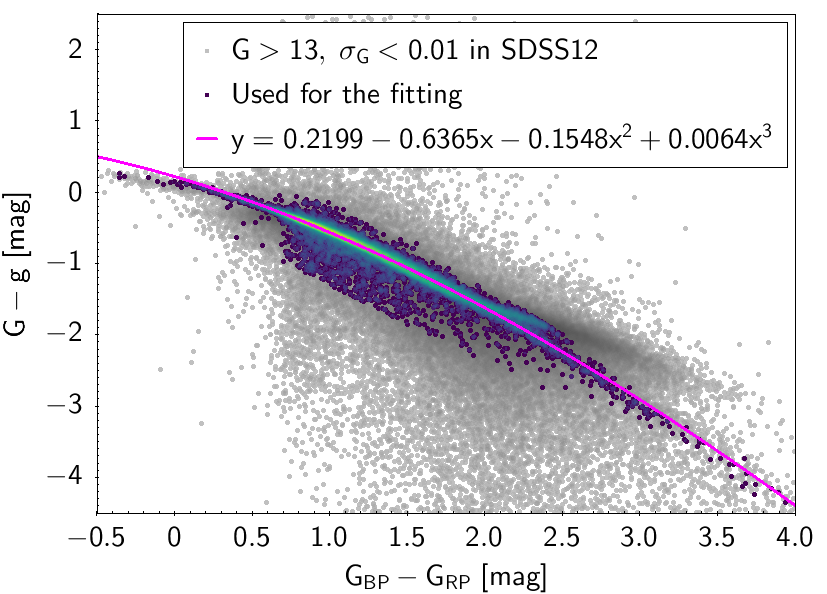
\includegraphics[scale=0.18]{Muestra/Secciones/Figures/Gaia-SDSS-Transform-g.png}
	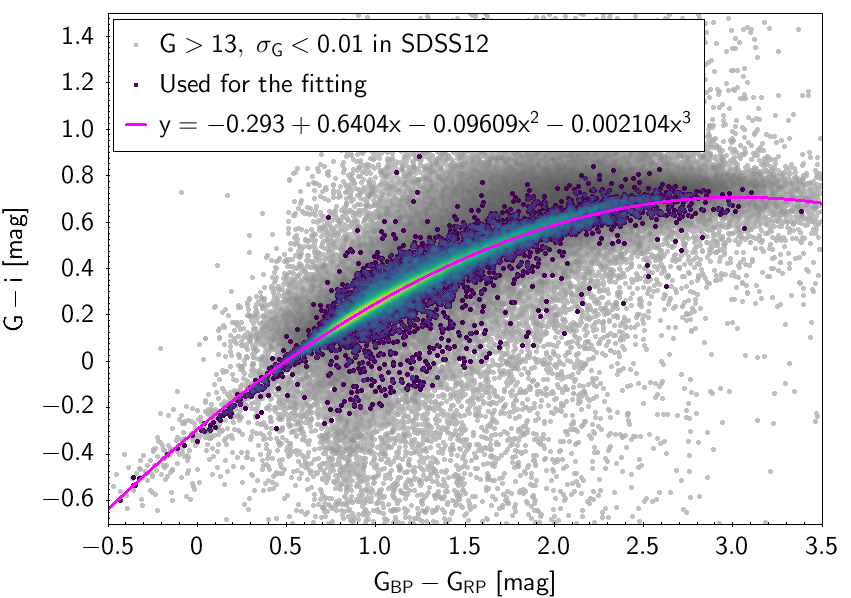
\includegraphics[scale=0.18]{Muestra/Secciones/Figures/Gaia-SDSS-Transform-i.png}
	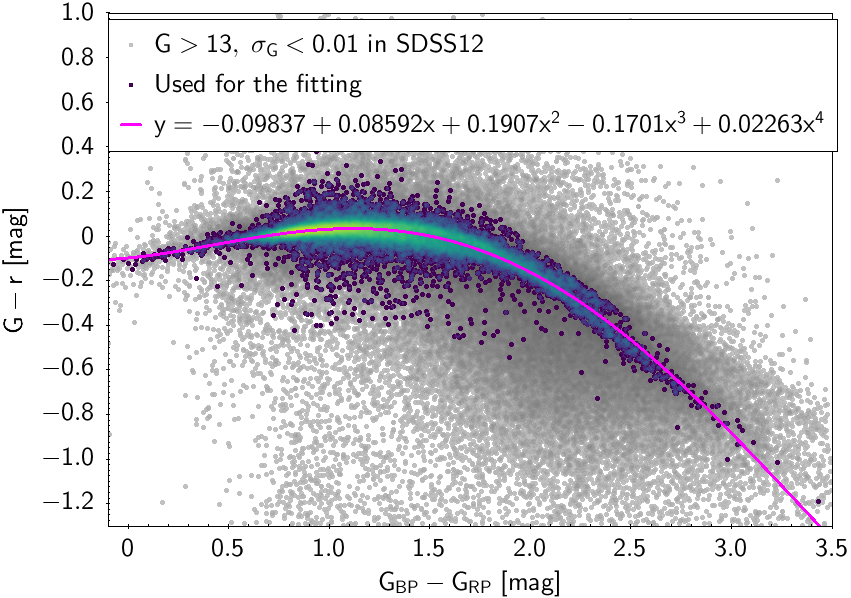
\includegraphics[scale=0.18]{Muestra/Secciones/Figures/Gaia-SDSS-Transform-r.png}

	\caption{Relación empírica entre las magnitudes reportadas en GDR3 y SDSS12. Las relaciones están dadas para 3 de las 5 bandas de SDSS12, debido a las diferencias entre las pasa bandas de Gaia y SDSS. \autocite{gdr3ReleaseDocumentation}}
	\label{gdr3SdssConversionGraphs}
\end{figure}

\section{Selección de Objetos Observables} \label{muestra:crit_seleccion:objetos_observables}

La ubicación en la bóveda celeste de un sistema candidata juega un papel
importante en la viabilidad de una campaña de observación desde el OAU. Esto
determina si un objeto es visible desde la locación geográfica del observatorio
durante las fechas de observación; de otra manera sería imposible apuntar un
telescopio al sistema. Para realizar esta tarea se utilizaron los módulos de
\code{astroplan} \autocite{astroplan} y \code{astropy} \autocite{astropy}, aplicando
el algoritmo a los objetos resultados de la búsqueda en la base de datos de
Gaia. El código responsable se encuentra en el archivo
\href{https://github.com/KnightIV/UANL_MAPTA_Observaciones/blob/main/obsrv_plan/gaia/observable_targets.py}{\code{observable\_targets.py}}.

% TODO: agrega resultados de cuantos objetos en total fueron elegidos?

\section{Búsqueda en SIMBAD} \label{muestra:crit_seleccion:busqueda_simbad}

% TODO: pregunta como referir al trabajo (presente o pasado? o hasta futuro?)
Una vez obtenidos los objetos de interés de la selección de objetos visibles se
utilizó la base de datos de
SIMBAD\footnote{\url{http://simbad.cds.unistra.fr/simbad/}}
\autocite{simbadDatabase} para restringir los objetos de interés a un tamaño
manejable, con el objetivo de obtener un sistema clasificado como variable
cataclísmica, binaria eclipsante, o candidata a alguna de estas clasificaciones.
Uno de los objetivos de este trabajo de tesis fue realizar una campaña de
observación al sistema elegido, con finalidad de obtener una curva de luz
fotométrica; por lo tanto, un requisito para este trabajo de maestría es que
este sistema sea uno con una cantidad minima de estudios antecedentes; el
estudio del sistema dependerá en gran parte de la curva de luz obtenida de las
observaciones. Esta búsqueda śe llevó a cabo utilizando el API de SIMBAD, el
cual acepta mensajes y encuestas por HTTP. El código relevante a esta búsqueda
se encuentra en
\href{https://github.com/KnightIV/UANL_MAPTA_Observaciones/blob/main/obsrv_plan/simbad/retrieve_vots.py}{\code{retrieve\_vots.py}}.
A pesar de no haber obtenido una muestra significativa de candidatas a binarias
eclipsante se identificó un sistema de interés.

% TODO: agrega histograma de SIMBAD